\documentclass{beamer}

\usepackage[utf8]{inputenc}
\usepackage[italian]{babel}
\usepackage{graphicx}
\usepackage[font=tiny,labelfont=bf]{caption}
\usepackage{hyperref}
\usepackage{tikz}

\hypersetup{colorlinks=true, linkcolor=black, urlcolor=blue}

\usetheme{Boadilla}

\graphicspath{ {./pics} }

\title[ML for SE]{Machine Learning for Software Engineering}
\subtitle{ISW2 project a.y. 2023/2024}
\author[Stefano Belli, 0350116]{Stefano Belli, matricola 0350116}
\institute[uniroma2]{Università degli Studi di Roma "Tor Vergata"}
\date{}

\usefonttheme[onlymath]{serif}

\newcommand{\dflvspace}{\vspace{10pt}}

\renewcommand{\footnotesize}{\tiny}

\setbeamertemplate{navigation symbols}{}
\setbeamertemplate{section in toc}{%
  {\color{blue!70!black}\inserttocsectionnumber.}~\inserttocsection}
\setbeamercolor{subsection in toc}{bg=white,fg=structure}
\setbeamertemplate{subsection in toc}{%
  \hspace{1.2em}{\color{blue}\rule[0.3ex]{3pt}{3pt}}~\inserttocsubsection\par}

\begin{document}

\begin{frame}[plain]
    \titlepage
\end{frame}

\begin{frame}
    \frametitle{Agenda}
    \fontsize{8pt}{10pt}\selectfont
    \tableofcontents
\end{frame}

\section{Introduzione}
\begin{frame}
	\frametitle{Introduzione}
	
	\begin{itemize}
		\setlength\itemsep{10pt}
	
		\item Nei grandi progetti software, il collaudo è cruciale: avere una buona test suite aiuta a prevenire
		malfunzionamenti spiacevoli per l'utente, permettendo il rilevamento del difetto prima della release.
	
		\item Tuttavia, eseguire numerosi test è dispendioso sia in termini di tempo d'esecuzione dei test sia per
		quanto riguarda la loro progettazione e implementazione: per quali unità conviene focalizzarsi?
		
		\item Per aiutarci a rispondere a questa domanda, possiamo sfuttare un modello di machine learning che 
		date informazioni sul codice sorgente, predica se l'unità in esame sia "buggy" o meno
		(e quindi, ci aiuti a decidere se generare dei test case per quest'ultima).
	\end{itemize}
\end{frame}

\section{Scopo}
\begin{frame}
	\frametitle{Scopo}
	
	\begin{itemize}
		\setlength\itemsep{10pt}
		
		\item Si vogliono confrontare le prestazioni di tre classificatori (Naive Bayes, IBk, Random Forest) con e
		senza tecniche di feature selection, sampling e cost sensitivity.
		\begin{itemize}
			\item Prediction della buggyness di una classe Java
		\end{itemize}
	
		\item Per la costruzione del dataset (e quindi la comparazione dei classificatori)
		vengono sfruttati i progetti open source Apache BookKeeper e Apache Storm.
	\end{itemize}
\end{frame}

\section{Metodologia}
\subsection{Recupero informazioni su release e tickets da Jira}
\begin{frame}
	\frametitle{Recupero informazioni su release e tickets da Jira}
	
	Dal bug tracker Jira, utilizzato dalla Apache Software Foundation, vengono scaricati, tramite
	la sua REST API, informazioni riguardo alle \underline{release} e ai \underline{ticket} che siano di tipo
	\textit{"bug"}, il cui stato sia \textit{"closed"} o \textit{"resolved"}, e la risoluzione \textit{"fixed"}
	
	\dflvspace
	
	Le informazioni (in particolare le date) su questi tipi di ticket serviranno 
	poi per determinare quali classi sono buggate, in quali release.
	
	\dflvspace

	In Jira, nell'oggetto JSON della risposta, per ogni ticket, sono di particolare interesse questi campi 
	(che ci permetteranno di capire le release affette dal bug):
	\begin{itemize}
		\item L'array \textit{fields.version}
		che contiene le informazioni sulle release affette dal bug (affected versions)
		\item La stringa \textit{fields.created} che è la data di apertura del ticket
		\item La stringa \textit{fields.resolutiondate} che è la data di risoluzione del bug
	\end{itemize}
\end{frame}

\subsection{Ciclo di vita del difetto}
\begin{frame}
	\frametitle{Ciclo di vita del difetto}
	
	\fontsize{10pt}{10pt}\selectfont
	
	Al fine di determinare le versioni affette dal bug, definiamo:
	\begin{itemize}
		\item L' \textbf{injected version} (\textit{IV})
		che è il numero di versione in cui è stato introdotto il bug
		\item L' \textbf{opening version} (\textit{OV}) 
		che è il numero di versione in cui è stato aperto il ticket relativo al bug (che è stato quindi rilevato)
		\item La \textbf{fixed version} (\textit{FV}) 
		che è il numero di versione in cui è stato risolto il bug
	\end{itemize}
	
	\begin{center}
	\begin{tikzpicture}
		\draw (0,0) -- (2,0);
		\draw[color=red] (2,0) -- (5,0);
		\draw[color=red] (5,0) -- (8,0);
		\draw[->] (8,0) -- (11,0);
		\draw[fill=red] (2,0) circle (2pt) 
							node[above]{\small{$IV$}} 
							node[below]{\tiny{$2$}};
		\draw[fill=red] (5,0) circle (2pt) 
							node[above]{\small{$OV$}}
							node[below]{\tiny{$5$}};
		\draw[fill=white] (8,0) circle (2pt) 
							node[above]{\small{$FV$}}
							node[below]{\tiny{$8$}};
	\end{tikzpicture}
	\end{center}
	
	Tutte e 3 le \textit{IV},\textit{OV} e \textit{FV} permettono di individuare il "ciclo di vita" completo del
	bug, che è presente da \textit{IV} (incluso) fino a \textit{FV} (escluso).
	\begin{alertblock}{Problema}
	Le API di Jira, forniscono sempre informazioni riguardo alla creazione del ticket e alla sua risoluzione
	(permettendo di determinare, rispettivamente: opening e fixed version), 
	ma non sempre rispetto alle affected versions, non permettendo sempre di individuare la injected version!
	\end{alertblock}
\end{frame}

\subsection{Utilizzo della tecnica proportion}
\begin{frame}
	\frametitle{Utilizzo della tecnica proportion}
	Se l'injected version non è nota, per un certo bug
	possiamo sfruttare il \textbf{proportion} per stimare l'\textit{IV}:
	
	\dflvspace
	
	\begin{align*}
	p = \frac{FV-IV}{FV-OV}\;\;\;\;\Rightarrow\;\;\;\;IV = FV - (FV - OV)\cdot p
	\end{align*}
	
	\dflvspace
	
	\begin{exampleblock}{Applicazione}
	A partire dai bug la cui \textit{IV} è nota, calcoliamo $p$ (prima formula). 
	Poi, avendo appena calcolato la costante di proporzionalità $p$, per il bug di cui
	\underline{non} si conosce \textit{IV}, si applica la seconda formula, in modo da determinarla.
	\end{exampleblock}
\end{frame}

\subsection{Metodi di utilizzo di proportion}
\begin{frame}
	\frametitle{Metodi di utilizzo di proportion}
	Viene utilizzato proportion con le tecniche:
	\begin{itemize}
		\item \textbf{Cold start}: se il numero di tickets utilizzabili ai fini del calcolo di $p$ è minore
		di 5, si calcola la media di $p$ sui ticket per ognuno dei seguenti progetti Apache: 
		Avro, OpenJPA, Syncope, Tajo e ZooKeeper. 
		Infine si effettua la mediana su queste 5 medie, ottenendoil valore di $p$ finale.
		\item \textbf{Incremental}: se il numero di tickets utilizzabili ai fini del calcolo di $p$ è maggiore o
		uguale a 5: $p$ è calcolato effettuando la media delle proporzionalità $p$ di tutti i bug precedenti 
		(che hanno \textit{IV})
		rispetto a quello considerato attualmente, di cui bisogna stimare \textit{IV}.
	\end{itemize}
\end{frame}

\subsection{Costruzione del dataset: metriche}
\begin{frame}
	\frametitle{Costruzione del dataset: metriche}
	
	\fontsize{9pt}{10pt}\selectfont
	
	% JGit, commit, releases unione info da jira e git
	\begin{itemize}
	
		\item Viene usato JGit al fine di poter manipolare un 
		repository Git direttamente tramite metodi Java: possiamo
		collezionare informazioni su commit e quindi anche sul codice sorgente 
		(esclusivamente classi Java) del repo di interesse.
		
		\item Dalle informazioni ricavate da Git, si possono calcolare delle metriche di interesse
		su un certo file Java che verranno poi utilizzate dal classificatore ai
		fini della predizione
	\end{itemize}
	
	\dflvspace
	
	Le metriche di interesse scelte sono le seguenti:
	
	\dflvspace
	
	\centering
	\begin{tabular}{|l|l|}
		\hline
		\textbf{Metrica} & \textbf{Descrizione} \\
		\hline
		\hline 
		LOC & Numero di linee di codice\\
		\hline
		LOC added & Somma di LOC aggiunte sulle revisioni\\
		\hline
		Avg. LOC added & Media di LOC aggiunte sulle revisioni\\
		\hline
		Max. LOC added & Numero massimo di LOC aggiunte tra le revisioni\\
		\hline
		Churn & Somma di LOC aggiunte e rimosse sulle revisioni\\
		\hline
		Avg. churn & Media di LOC aggiunte e rimosse sulle revisioni\\
		\hline
		Max. churn & Numero massimo di LOC aggiunte e rimosse tra le revisioni\\
		\hline
		Avg. chg. set & Media di file cambiati insieme sulle revisioni\\
		\hline
		Max. chg. set & Numero massimo di file cambiati insieme sulle revisioni\\
		\hline
		Num. of authors & Numero di autori\\
		\hline
		Num. of revs & Numero di revisioni\\
		\hline
	\end{tabular}
	
	
\end{frame}

\subsection{Costruzione del dataset: buggyness e snoring}
\begin{frame}
	\frametitle{Costruzione del dataset: buggyness e snoring}
	
	\begin{itemize}
		\item Le informazioni ottenute da Jira vengono "collegate" a quelle ricavate da Git (ticket e release vengono 
		associati ai commit).
		
		\item Il dataset, oltre ad essere composto dalle metriche di interesse appena elencate, 
		ha nella prima e seconda colonna rispettivamente
		la versione del progetto Apache in esame, il path al file Java interessato , nel mezzo le metriche,
		e come ultima colonna la buggyness.
		
		\item La \textbf{buggyness}
		(variabile binaria che può assumere valore "YES" o "NO" e che il classificatore deve predirre) viene 
		determinata grazie al collegamento delle informazioni ricavate tra Jira e Git.
		\begin{itemize}
			\item Una classe Java è \textit{buggy} se la versione $v$ in cui ricade è compresa nell'intervallo 
			$IV \le v < FV$
		\end{itemize}
	\end{itemize}
	
	\begin{alertblock}{Snoring}
	Al fine di ridurre l'effetto dello \textbf{snoring}, ovvero bug dormienti non rilevati, sono stati eliminati
	tutti i dati relativi alla seconda metà delle releases. Dare in pasto al classificatore dati affetti da
	snoring può comprometterne le prestazioni.
	\end{alertblock}
	
\end{frame}

\subsection{Classificatori e tecniche considerate}
\begin{frame}
	\frametitle{Classificatori e tecniche considerate}
	
	\fontsize{7pt}{8pt}\selectfont
	
	Sono stati utilizzati 3 classificatori diversi\dots
	\begin{itemize}
		\item Random forest
		\item Naive Bayes
		\item IBk
	\end{itemize}
	
	\begin{columns}[T]
		\begin{column}{0.5\linewidth}
		\dots ognuno con le seguenti tecniche\dots
		
		\textbf{Feature selection}
		\begin{itemize}
			\item Nessuna tecnica di feature selection
			\item Best first backward
		\end{itemize}
	
		\textbf{Sampling}
		\begin{itemize}
			\item Nessuna tecnica di sampling
			\item SMOTE
			\item Undersampling
		\end{itemize}
	
		\textbf{Cost sensitivity}
		\begin{itemize}
			\item Nessuna tecnica di cost sensitivity
			\item Sensitive Learning
		\end{itemize}
		\end{column}
	
		\begin{column}{0.5\linewidth}
		\dots combinate come segue:
		\begin{tabular}{|c|}
			\hline
			Nessuna tecnica utilizzata\\
			\hline
			Solo sensitive learning\\
			\hline
			Solo best first backward\\
			\hline
			Solo undersampling\\
			\hline 
			Solo SMOTE\\
			\hline
			Best first backward e sens. learning\\
			\hline
			Best first backward e undersampling\\
			\hline
			Best first backward e SMOTE\\
			\hline
		\end{tabular}
		\end{column}
	\end{columns}
	\dflvspace
	La \underline{valutazione} viene effettuata tramite l'ausilio 4 metriche: 
	\textbf{F1-score} 
	(media armonica tra precision e recall, il cui valore sta nel range $[0,1]$: 
	è 1 se lo sono sia precision che recall, è 0 alla condizione che lo siano sia precision che recall),
	\textbf{Kappa}, \textbf{AUC}, 
	\textbf{NPofB20} (percentuale di bug che
	possono essere trovati analizzando il top 20\% di LOC. Il ranking, per definire
	il \textit{"top 20\% di LOC"}
	è effettuato sulla prob. pred. di buggyness diviso la size della classe).
	
	Ne viene valutato, inoltre, il \textbf{costo}: $CFN \cdot FN + CFP \cdot FP$ con
	$CFN=10,\;CFP=1$
\end{frame}

\subsection{Evaluation con walk forward}
\begin{frame}
	\frametitle{Evaluation con walk forward}
	
	\fontsize{8pt}{10pt}\selectfont
	
	Lo strumento utilizzato per valutare le prestazioni dei classificatori (con o senza tecniche) è
	una tecnica di tipo time-series: walk forward.
	
	\begin{itemize}
		\item Nella figura sottostante è presente un esempio di esecuzione dell'evaluation: ogni cella,
		rappresenta i dati relativi alla release $i-$esima (dove $i$ è la colonna di appartenenza) 
		e la colorazione indica la split che viene attuata alla $j-$esima iterazione (dove $j$ è la riga)
	
		\item Nel nostro caso, la prima run, non viene effettuata a prescindere dato che non abbiamo un training set con cui addestrare
		un classificatore e quindi viene ritenuta inutile.
		\item Le run per BookKeeper partono dalla run 3 
		(2 training rels. + 1 testing rel), 
		mentre le run per Storm partono dalla run 4 (3 training rels.  + 1 testing rel.)
		\begin{itemize}
			\fontsize{7pt}{10pt}\selectfont
			\item Essendo una tecnica time-series, i dati disponibili fino alle release di training non rivelano
			alcuna classe buggy, impedendo l'addestramento del classificatore
		\end{itemize}
	\end{itemize}
	
	\begin{center}
	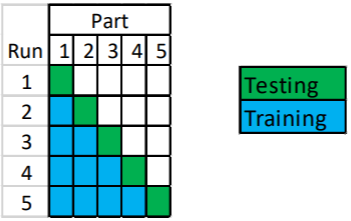
\includegraphics[width=4cm, height=2.25cm]{walkforward}
	\end{center}
	
	\fontsize{8pt}{10pt}\selectfont
	
	Il \textbf{training set} deve riflettere l'utilizzo reale del classificatore, 
	può essere affetto da snoring: non utilizziamo i dati del futuro per determinare 
	la buggyness (la tecnica è time-series), al contrario, per il \textbf{testing set}
	vengono utilizzati tutti i dati a nostra disposizione, deve essere
	il più accurato possibile e non deve essere affetto da snoring (idealmente)
\end{frame}

\section{Risultati}
\subsection{Risultati per BookKeeper}
\begin{frame}
	\frametitle{Risultati per BookKeeper: F1-score}
	
	\fontsize{7pt}{8pt}\selectfont
	
	Tra tutte le soluzioni proposte, \textbf{IBk no
	feature selection, si SMOTE, no cost sensitivity, ha l'F1-score migliore}.
	
	\centering
	\begin{figure}
	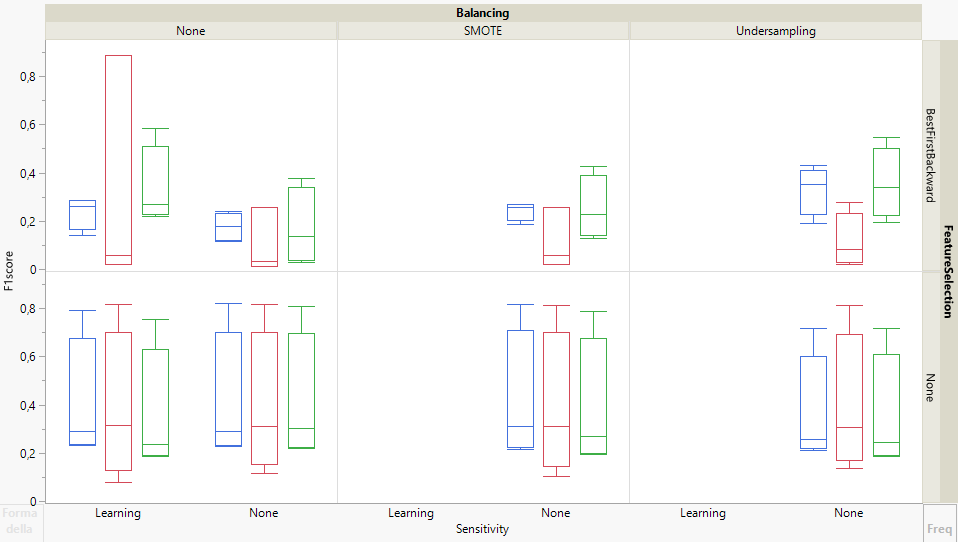
\includegraphics[width=10cm, height=6cm]{bookkeeper-f1score}
	\caption{Il box plot verde è per Random forest, rosso per Naive Bayes, blu per IBk}
	\end{figure}
\end{frame}

\begin{frame}
	\frametitle{Risultati per BookKeeper: Kappa}
	
	\fontsize{7pt}{8pt}\selectfont
	
	I kappa peggiori sono sicuramente quelli di Naive Bayes 
	senza feature selection con SMOTE (no cost sensitivity), Naive Bayes senza
	applicazione di feature selection, senza balancing, no cost sensitivity e 
	Naive Bayes senza applicazione di feature selection, senza balancing, sens.
	learning.
	\textbf{IBk si feature 
	selection, no balancing, no cost sensitivity, ha il kappa migliore} 
	(anche se IBk, si feature selection, no balancing, si sens. learning, 
	non sembra essere male: il valore massimo è inferiore, ma non troppo e
	rispetto al precedente ha un valore minimo e mediana leggermente più alti)
	
	\centering
	\begin{figure}
	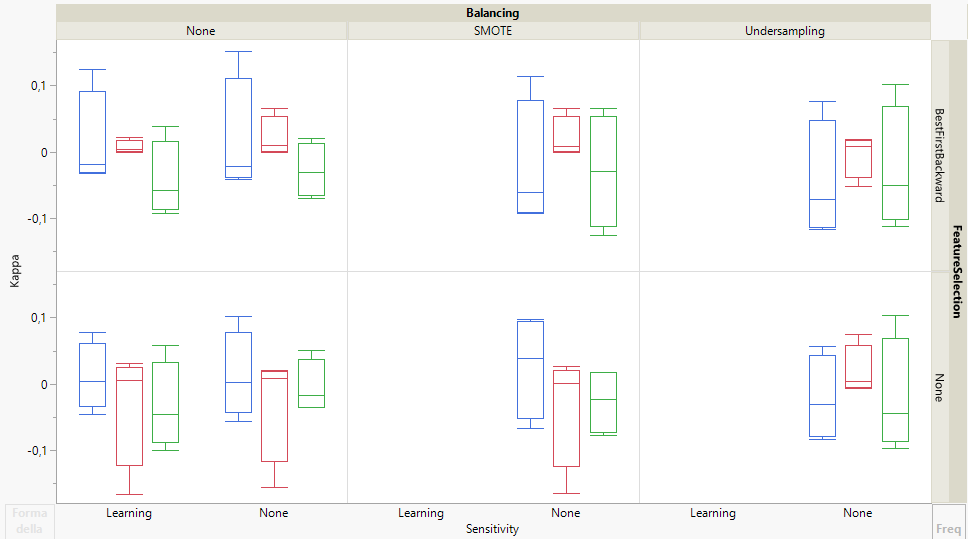
\includegraphics[width=10cm, height=6cm]{bookkeeper-kappa}
	\caption{Il box plot verde è per Random forest, rosso per Naive Bayes, blu per IBk}
	\end{figure}
\end{frame}

\begin{frame}
	\frametitle{Risultati per BookKeeper: AUC}
	
	\fontsize{7pt}{8pt}\selectfont
	
	Naive Bayes sembra essere quello che ha i valori massimi più alti, ma anche i
	valori minimi e mediane più bassi.
	Per quanto riguarda IBk, la mediana è decisamente più elevata rispetto agli
	altri due classificatori, con tutte le combinazioni delle tecniche.
	\textbf{Random forest, no feature selection, si SMOTE, no cost sensitivity,
	ha l'AUC migliore}.
	
	\centering
	\begin{figure}
	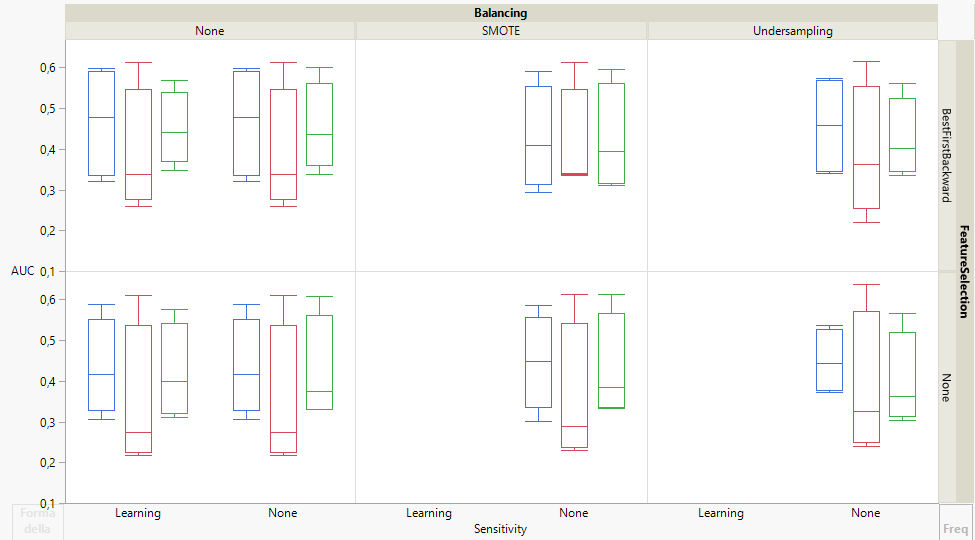
\includegraphics[width=10cm, height=6cm]{bookkeeper-auc}
	\caption{Il box plot verde è per Random forest, rosso per Naive Bayes, blu per IBk}
	\end{figure}
\end{frame}

\begin{frame}
	\frametitle{Risultati per BookKeeper: NPofB20}
	
	\fontsize{7pt}{8pt}\selectfont
	
	In generale, l'applicazione di feature selection peggiora NPofB20 per tutti i
	classificatori e le possibili combinazioni di balancing e cost sensitivity
	(tutti i 3 riquadri sopra).
	\textbf{IBk, no feature selection, si SMOTE, no cost sensitivity, ha l'
	NPofB20 migliore} (nonostante altri classificatori riescono ad ottenere risultati
	simili in termini di massimo, riesce ad avere minimo e mediana più alti).
	
	\centering
	\begin{figure}
	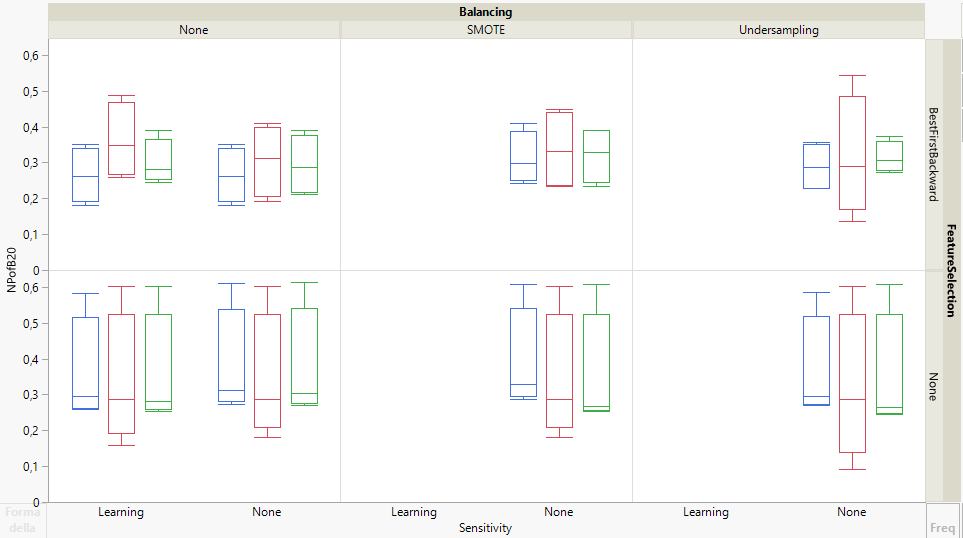
\includegraphics[width=10cm, height=6cm]{bookkeeper-npofb20}
	\caption{Il box plot verde è per Random forest, rosso per Naive Bayes, blu per IBk}
	\end{figure}
\end{frame}

\begin{frame}
	\frametitle{Risultati per BookKeeper: costi}
	
	\fontsize{7pt}{8pt}\selectfont
	
	Risulta chiaro che l'applicazione di feature selection incrementa notevolmente il costo.
	\textbf{Random forest senza l'applicazione di alcuna tecnica è il classificatore con il
	costo più basso}
	
	\centering
	\begin{figure}
	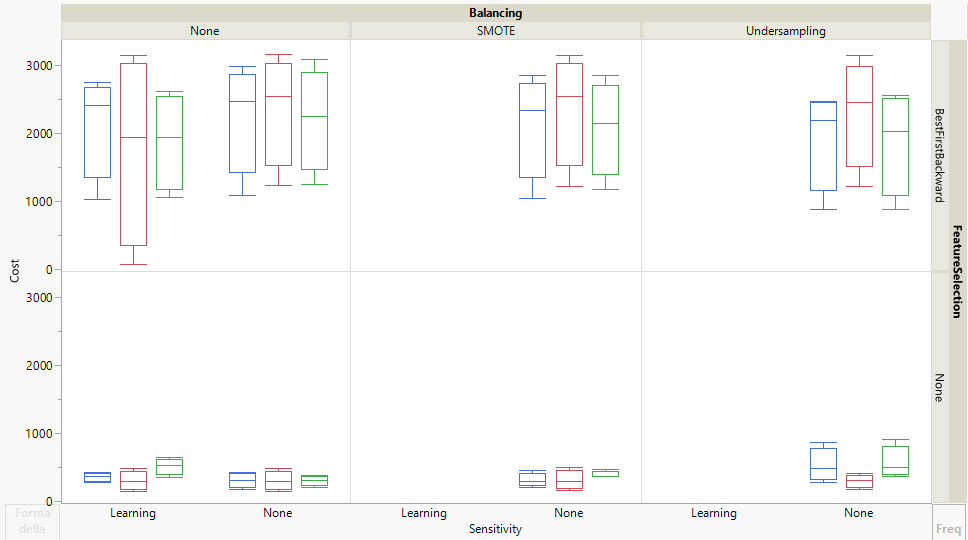
\includegraphics[width=10cm, height=6cm]{bookkeeper-cost}
	\caption{Il box plot verde è per Random forest, rosso per Naive Bayes, blu per IBk}
	\end{figure}
\end{frame}

\subsection{Risultati per Storm}
\begin{frame}
	\frametitle{Risultati per Storm: F1-score}
	
	\fontsize{7pt}{8pt}\selectfont
	
	Tutti i classificatori, di tutte le combinazioni presentano, più o meno, lo stesso minimo.	
	L'applicazione di feature selection sembra migliorare notevolmente il massimo assunto dai classificatori.
	In combinazione al feature selection, utilizzare sensitive learning migliora notevolmente la metrica 
	F1-score, e quello con punteggio più alto è IBk o Random forest.
	A parità di minimo, \textbf{Random forest, si feature selection, no balancing, si sens. learning, risulta
	essere quello con punteggio F1 più alto}, ma con le stesse identiche tecniche applicate, anche IBk non
	è male: viene scelto RF solo perchè ha massimo e mediana più alti.
	
	\centering
	\begin{figure}
	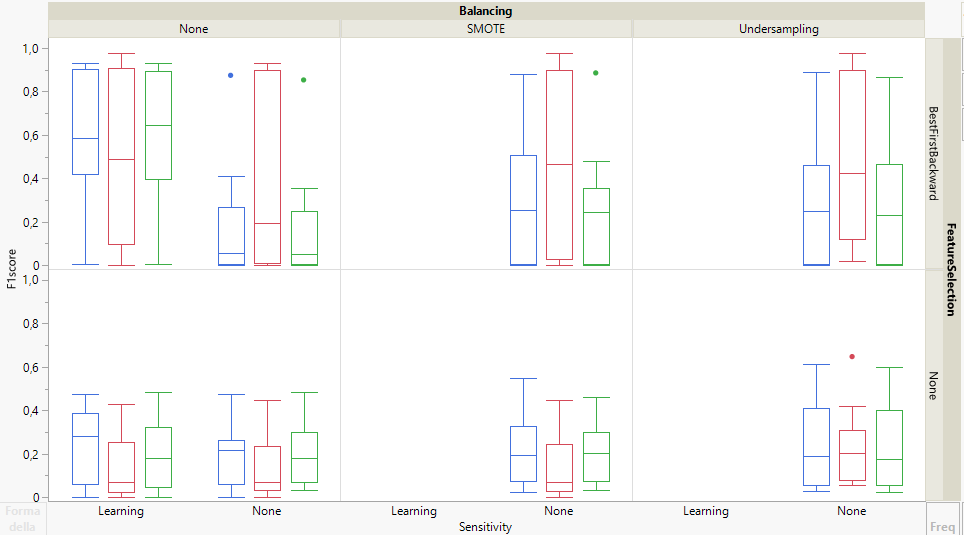
\includegraphics[width=10cm, height=6cm]{storm-f1score}
	\caption{Il box plot verde è per Random forest, rosso per Naive Bayes, blu per IBk}
	\end{figure}
\end{frame}

\begin{frame}
	\frametitle{Risultati per Storm: Kappa}
	
	\fontsize{7pt}{8pt}\selectfont
	
	Il sensitive learning si riconferma una tecnica molto efficace, in particolare con IBk.
	
	Con un outlier $> 0.4$, 
	\textbf{IBk, si feature selection, no balancing, si sensitive learning è la combinazione che fornisce
	kappa migliore}. Si distingue anche la stessa configurazione, ma senza feature selection (di fatto, molto
	simili).
	
	\centering
	\begin{figure}
	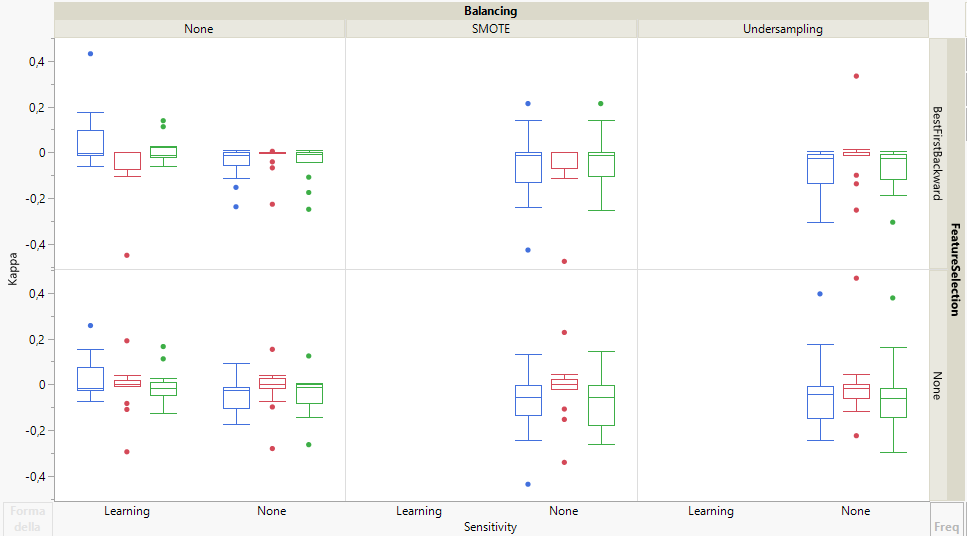
\includegraphics[width=10cm, height=6cm]{storm-kappa}
	\caption{Il box plot verde è per Random forest, rosso per Naive Bayes, blu per IBk}
	\end{figure}
\end{frame}

\begin{frame}
	\frametitle{Risultati per Storm: AUC}
	
	\fontsize{7pt}{8pt}\selectfont
	
	Per quasi tutte le combinazioni, IBk risulta essere il migliore in termini di AUC.
	
	Tutti i box plot riguardanti AUC di IBk sono a loro volta simili, ad eccezione per l'undersampling.
	
	\underline{Scelto} IBk e 
	\underline{scartate} le configurazioni che hanno come balancing l'undersampling, si possono anche
	\underline{scartare} quelle che non hanno applicato feature selection 
	(i minimi sono gli stessi, i massimi più
	bassi, rispetto alle configurazioni che applicano feature selection).
	
	\textbf{IBk, si feature selection, no balancing, si sensitive learning, risulta essere quello con AUC
	migliore}
	
	\centering
	\begin{figure}
	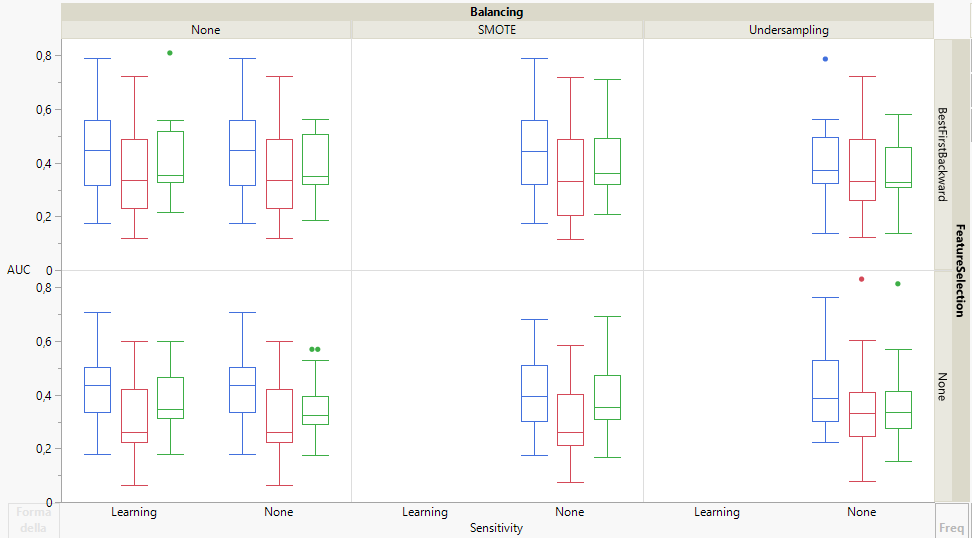
\includegraphics[width=10cm, height=6cm]{storm-auc}
	\caption{Il box plot verde è per Random forest, rosso per Naive Bayes, blu per IBk}
	\end{figure}
\end{frame}

\begin{frame}
	\frametitle{Risultati per Storm: NPofB20}
	
	\fontsize{7pt}{8pt}\selectfont
	
	\textbf{Random forest, si feature selection, no balancing, no sens. learning ha l'NPofB20 migliore}
	
	\centering
	\begin{figure}
	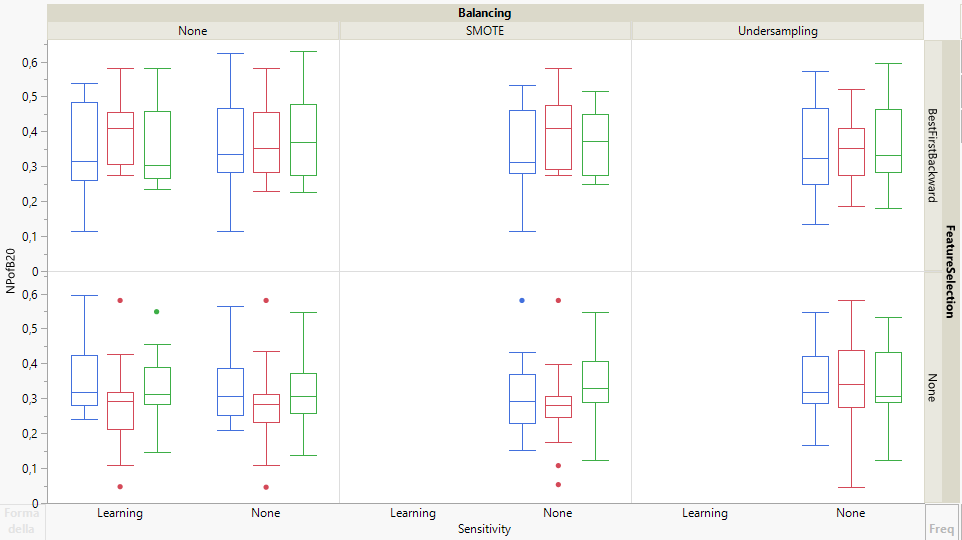
\includegraphics[width=10cm, height=6cm]{storm-npofb20}
	\caption{Il box plot verde è per Random forest, rosso per Naive Bayes, blu per IBk}
	\end{figure}
\end{frame}

\begin{frame}
	\frametitle{Risultati per Storm: costi}
	
	\fontsize{7pt}{8pt}\selectfont
	
	\textbf{IBk, no feature selection, no balancing, si sens. learning ha il costo migliore 
	(tendenzialmente più basso)}
	
	\centering
	\begin{figure}
	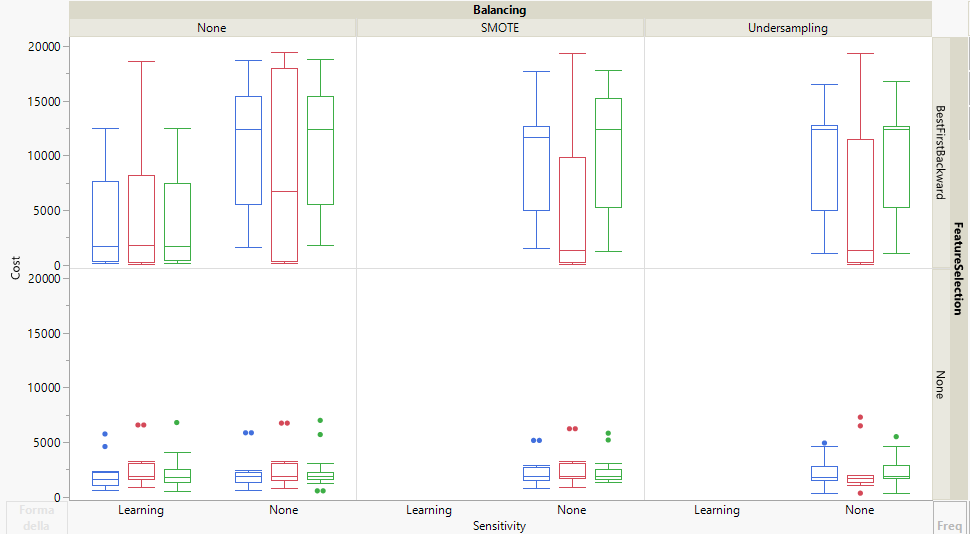
\includegraphics[width=10cm, height=6cm]{storm-cost}
	\caption{Il box plot verde è per Random forest, rosso per Naive Bayes, blu per IBk}
	\end{figure}
\end{frame}

\section{Conclusioni e minacce alla validità}
\begin{frame}
	\frametitle{Conclusioni e minacce alla validità}
	
	\fontsize{7pt}{8pt}\selectfont
	
	\textbf{Conclusioni}
	
	\begin{itemize}
		\item 
		Non esiste una scelta migliore dell'altra, tuttavia, possiamo affermare che per BookKeeper una scelta
		non da fare è sicuramente usare Naive Bayes e mentre IBk ottiene complessivamente metriche migliori, per
		Random Forest si tende a registrare un costo più basso. \textbf{Una eventuale scelta comunque, ricadrebbe su IBk,
		con la sola applicazione di balancing (SMOTE)}, dato che l'F1-score è il migliore, 
		mentre kappa e AUC non sono le
		migliori, ma nemmeno le peggiori (si preferisce un F1-score più alto).
		La scelta di IBk con la sola applicazione di SMOTE è confermata da NPofB20.
		C'è comunque da ricordare che
		i dati, e il numero di iterazioni di walk forward per BookKeeper è basso, a causa delle poche release
		a disposizione.
		
		\item
		In Storm, conviene sempre scartare Naive Bayes, e per quasi tutte le metriche, usare IBk o Random forest
		con la configurazione:
		feature selection (best first backward), niente balancing e cost sensitivity (sensitive learning).
		Mantenendo la preferenza per un F1-score alto, ma anche tenendo in considerazione kappa, AUC e costi,
		\textbf{conviene sicuramente utilizzare IBk con feature selection (best first backward), no balancing e 
		con cost sensitivity (sensitive learning)}, che rappresenta un buon compromesso per le metriche e il costo
		considerati. 
		NPofB20 tende a favorire Random forest (si feature selection, no balancing, no sens. learning),
		ma AUC e Kappa e la poca differenza per l'F1-score, sposta l'ago della bilancia a favore di IBk con le
		tecniche scelte.
		I dati a disposizione e il numero di release elevati ha sicuramente permesso di ottenere dei risultati più
		affidabili rispetto a BookKeeper.
	\end{itemize}
	
	\textbf{Minacce alla validità}
	
	\begin{itemize}
		\item Si assume che le informazioni prelevate da Jira siano affidabili
		\item Le release e i ticket senza commit vengono scartati
	\end{itemize}
	
\end{frame}

\section{Links}
\begin{frame}
	\frametitle{Links}
	
	\begin{itemize}
		\item GitHub: \url{https://github.com/StefanoBelli/isw2-deliverable}
		\item SonarCloud: \url{https://sonarcloud.io/project/overview?id=StefanoBelli_isw2-deliverable}
	\end{itemize}
	
\end{frame}

\begin{frame}[noframenumbering, plain]
    \frametitle{}
    
    \fontsize{30pt}{10pt}\selectfont
    \centering
    \textbf{Grazie per l'attenzione!}
    
\end{frame}


\end{document}
